% 问题三完整正文。需要宏包：amsmath, amssymb, graphicx, booktabs, multirow。
% 主性能结果全部来自冻结 test；validation 仅用于选择，未作为最终性能。

\section{问题三的建模分析与求解}
\label{sec:q3}

\subsection{问题描述与任务分析}

问题三要求利用附件2中已经对齐的文本、语音和视觉序列，同时预测情感极性与连续情感强度，并解释每个样本的主要参考模态和关键局部证据。令模态集合为
\(\mathcal M=\{T,A,V\}\)，第 \(i\) 个样本的输入为
\begin{equation}
X_i^m\in\mathbb R^{L\times d_m},\qquad
L=50,\quad (d_T,d_A,d_V)=(768,74,35),
\label{eq:q3_input}
\end{equation}
其中 74 维语音和 35 维视觉仅表示赛题提供的时序特征，不对单个维度赋予未经赛题或代码证实的物理含义。分类标签
\(c_i\in\{\mathrm{Negative},\mathrm{Neutral},\mathrm{Positive}\}\) 与连续标签 \(y_i\in[-3,3]\) 满足严格符号关系：\(y_i<0\) 为 Negative，\(y_i=0\) 为 Neutral，\(y_i>0\) 为 Positive。

该任务存在四个难点：第一，三种模态的维数、噪声和信息密度不同；第二，情感证据只集中在部分对齐位置；第三，模态之间既可能一致，也可能发生冲突；第四，注意力可视化本身不能说明某项证据真实影响最终决策。为此，我们将问题分成“基础可解释表征”和“最终稳健部署”两层：基础 C$^3$-HAFusion 学习时序、冲突和动态贡献；最终 EXP183 使用七个异构成员形成固定共识，再对父模型判为 Neutral 的样本执行真实性仲裁。最终解释直接作用于冻结部署图，而不是用某个成员的注意力替代集成模型解释。

\begin{table}[htbp]
\centering
\caption{三模态输入特征}
\label{tab:q3_input_features}
\small
\resizebox{\textwidth}{!}{%
\begin{tabular}{lrrrr}
\toprule
Modality & Symbol & Length & Dimension & Description \\
\midrule
Text & X(T) & 50 & 768 & Competition-provided aligned textual representation \\
Audio & X(A) & 50 & 74 & Competition-provided aligned acoustic representation \\
Vision & X(V) & 50 & 35 & Competition-provided aligned visual representation \\
\bottomrule
\end{tabular}%
}
\end{table}


\subsection{数据审计与总体建模思路}

数据划分包含 3395 个训练样本、728 个验证样本和 727 个测试样本。审计未发现跨划分样本 ID、视频组或完整特征哈希重叠，未发现 NaN/Inf，也未发现分类标签与连续标签符号冲突。视觉全零样本在 train/validation/test 中分别为 110/15/28；原始文本 padding 仍有预训练表示，但归一化器在进入模型前按有效掩码清零。

\begin{table}[htbp]
\centering
\caption{数据集划分及类别分布}
\label{tab:q3_dataset_split}
\small
\resizebox{\textwidth}{!}{%
\begin{tabular}{lrrrr}
\toprule
Split & Negative & Neutral & Positive & Total \\
\midrule
train & 967 & 758 & 1670 & 3395 \\
valid & 206 & 184 & 338 & 728 \\
test & 207 & 158 & 362 & 727 \\
\bottomrule
\end{tabular}%
}
\end{table}

\begin{table}[htbp]
\centering
\caption{连续标签统计}
\label{tab:q3_label_statistics}
\small
\resizebox{\textwidth}{!}{%
\begin{tabular}{lrrrrr}
\toprule
Split & mean & std & min & median & max \\
\midrule
train & 0.1658 & 1.1151 & -3.0000 & 0.0000 & 3.0000 \\
valid & 0.1609 & 1.0436 & -3.0000 & 0.0000 & 3.0000 \\
test & 0.1412 & 1.1581 & -3.0000 & 0.0000 & 3.0000 \\
\bottomrule
\end{tabular}%
}
\end{table}


\begin{figure}[htbp]
  \centering
  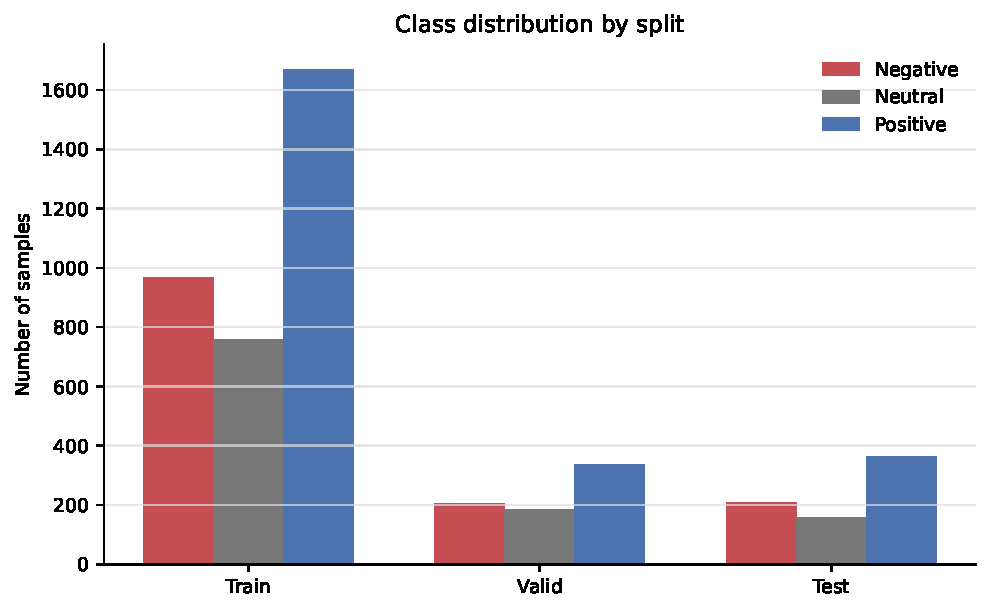
\includegraphics[width=0.49\textwidth]{../figures/fig_q3_class_distribution.pdf}
  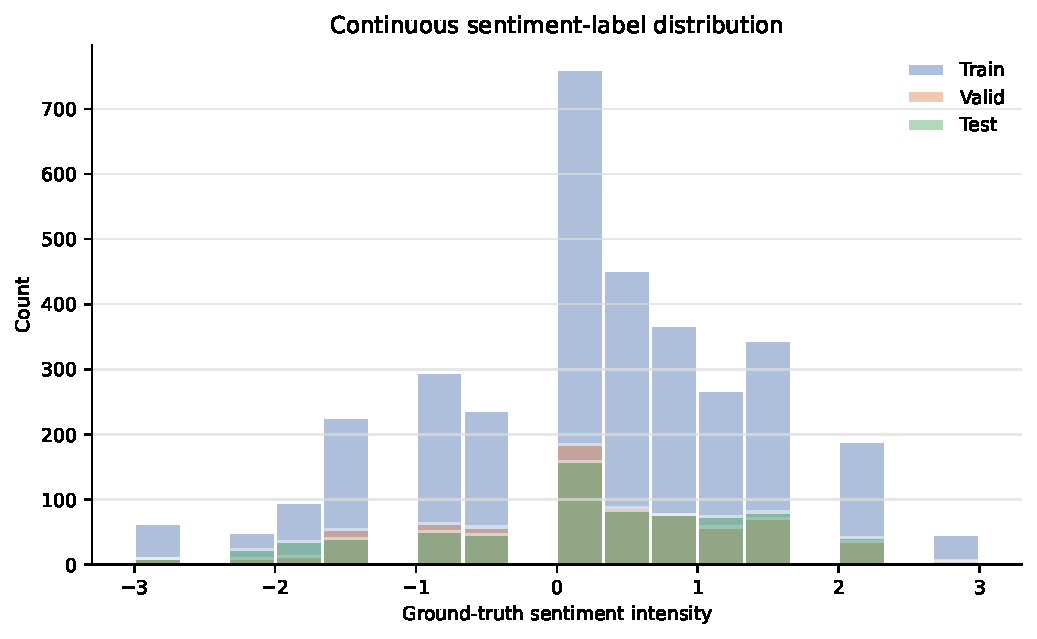
\includegraphics[width=0.49\textwidth]{../figures/fig_q3_intensity_distribution.pdf}
  \caption{数据集类别分布与连续情感强度分布}
  \label{fig:q3_data_distribution}
\end{figure}

图~\ref{fig:q3_framework} 给出总体流程。训练阶段只用 train 学习参数，并用 validation 选择 checkpoint 和冻结阈值；test 在 EXP183 完全冻结后读取一次，用于正式报告。后续 test 遮挡与删除仅用于解释已冻结模型，不再选择结构或超参数。

\begin{figure}[htbp]
  \centering
  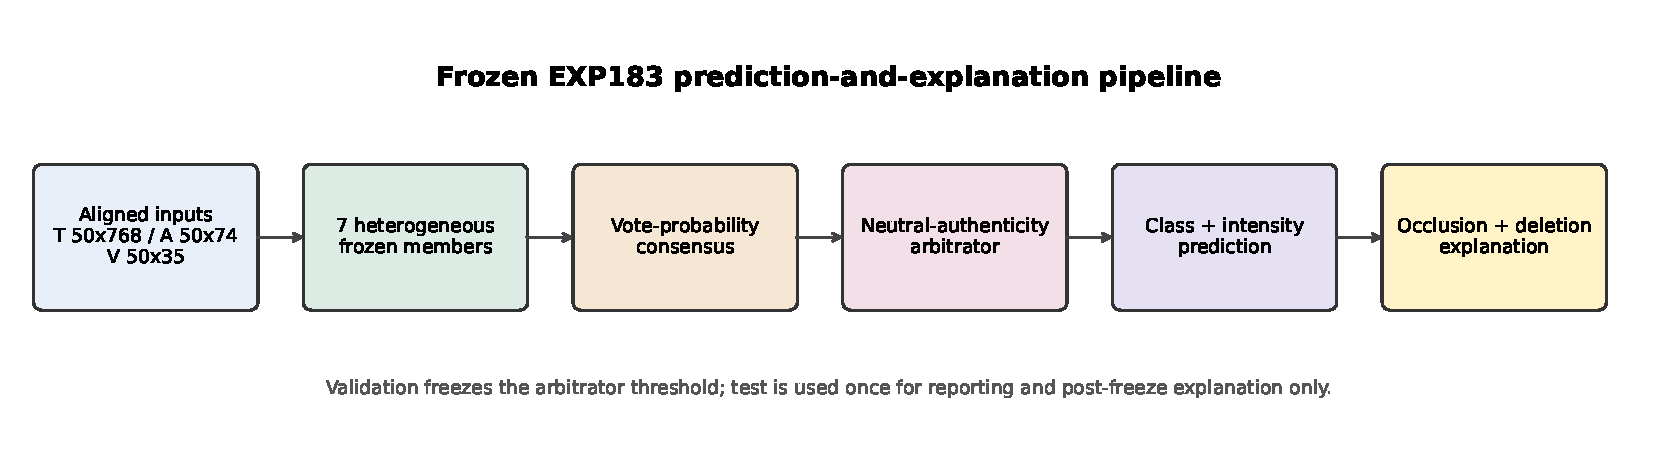
\includegraphics[width=\textwidth]{../figures/fig_q3_framework.pdf}
  \caption{问题三冻结预测与解释总体框架}
  \label{fig:q3_framework}
\end{figure}

\subsection{C$^3$-HAFusion 基础可解释模型}

\subsubsection{统一表征与模态内时序编码}

由文本 attention-mask 得到有效位置掩码 \(M_{i,t}\in\{0,1\}\)，并将该掩码复制到三种已对齐模态。每种模态先执行输入 LayerNorm 和线性映射，再加入正弦位置编码：
\begin{equation}
H_i^m=\operatorname{LN}_{\mathrm{out}}^m\!\left(
\operatorname{Transformer}_m\left(
\Phi_m(X_i^m)+\rho_m\operatorname{MSC}_m(\Phi_m(X_i^m))
\right)\right),
\label{eq:q3_temporal}
\end{equation}
其中 \(\Phi_m\) 包含输入归一化、线性投影、位置编码和 dropout，\(\operatorname{MSC}_m\) 是核大小为 3 和 5 的深度可分离一维卷积残差，Transformer 为两层、六头、pre-norm 结构。所有注意力、卷积输出和池化均乘有效掩码，padding 不参与决策。

\subsubsection{一致性与冲突关系}

对模态对 \((m,n)\)，先把两个流投影到公共空间。位置 \(t\) 的余弦相似度、一致程度和冲突程度分别为
\begin{equation}
s_{i,t}^{mn}=\cos(u_{i,t}^m,u_{i,t}^n),\quad
a_{i,t}^{mn}=\operatorname{clip}\!\left(\frac{s_{i,t}^{mn}+1}{2},0,1\right),\quad
d_{i,t}^{mn}=1-a_{i,t}^{mn}.
\label{eq:q3_conflict}
\end{equation}
据此构造
\begin{align}
q_{i,t}^{mn}&=a_{i,t}^{mn}\frac{u_{i,t}^m+u_{i,t}^n}{2},\\
r_{i,t}^{mn}&=d_{i,t}^{mn}\operatorname{MLP}_{mn}
\left([|u_{i,t}^m-u_{i,t}^n|;u_{i,t}^m-u_{i,t}^n]\right).
\label{eq:q3_pair}
\end{align}
一致部分 \(q^{mn}\) 保留共同证据，冲突部分 \(r^{mn}\) 同时保留差异幅度和方向；随后再乘由 MLP--sigmoid 估计的 pair 可靠性。因此模型不是直接拼接三模态，而是把三个单模态流和三个模态对流共同作为六个证据组件。

\subsubsection{局部证据与层次自适应融合}

对每个组件 \(j\)，EvidenceHead 将内容得分、局部结构相似度和显著性组合为位置分数 \(e_{i,t}^{j}\)，经 sparsemax 或 softmax 得到
\begin{equation}
\alpha_{i,t}^{j}=
\frac{M_{i,t}^{j}\exp(e_{i,t}^{j})}
{\sum_{s=1}^{L}M_{i,s}^{j}\exp(e_{i,s}^{j})},qquad
z_i^j=\sum_{t=1}^{L}\alpha_{i,t}^{j}h_{i,t}^{j}.
\label{eq:q3_local_pool}
\end{equation}
六个组件先做共享--私有正交分解，再通过可靠性调制的组件 self-attention 交换上下文。组件门控使用组件表示、全局均值、绝对差、乘积和可靠性作为输入，经 masked softmax 得到 \(g_i^j\ge0\) 且 \(\sum_jg_i^j=1\)。每个 pair 门以 0.5/0.5 分配给两个所属模态，因此三模态内部作用权重满足
\begin{equation}
I_i^m=g_{i,\mathrm{unary}(m)}+
\frac12\sum_{j:\,m\in j}g_i^j,qquad
\sum_{m\in\mathcal M}I_i^m=1.
\label{eq:q3_modality_gate}
\end{equation}
这里的 \(I_i^m\) 是模型内部动态权重，不直接解释为因果贡献；其可信度还需由最终管线遮挡检验。

\subsubsection{分类与回归联合预测}

六个组件分别给出局部分类和回归证据，经过分类--回归耦合、门控和 pair 分配形成三模态可加贡献 \(C_i^m\) 与 \(R_i^m\)。最终输出为
\begin{align}
o_i&=b_c+\sum_{m\in\mathcal M}C_i^m,\qquad
p_i=\operatorname{softmax}(o_i),\\
\hat y_i&=3\tanh\!\left(\frac{b_r+\sum_{m\in\mathcal M}R_i^m}{3}\right),
\label{eq:q3_prediction}
\end{align}
从而严格保证 \(\hat y_i\in[-3,3]\)。

C$^3$ 的代码定义为 Conflict-aware、Conservative 和 Counterfactually calibrated，即冲突感知、保守残差与反事实校准；本文不把它强行改写为代码没有正式声明的其他全称。HAFusion 表示层次自适应融合：先在位置层聚合，再在组件层交互，最后在模态层得到贡献。

\begin{figure}[htbp]
  \centering
  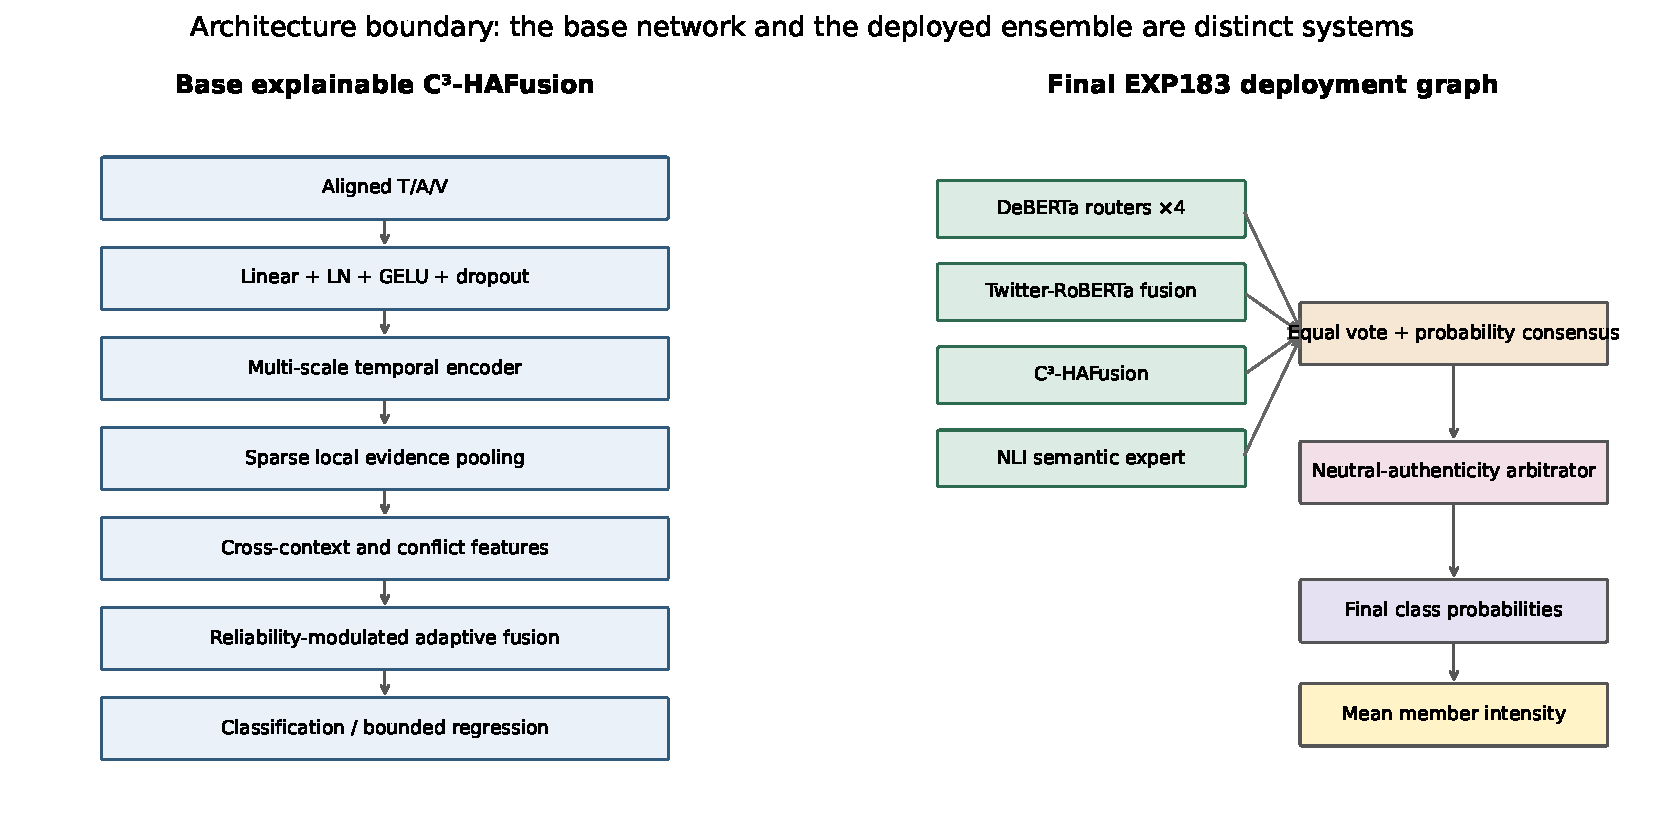
\includegraphics[width=\textwidth]{../figures/fig_q3_architecture.pdf}
  \caption{基础 C$^3$-HAFusion 与最终 EXP183 部署结构边界}
  \label{fig:q3_architecture}
\end{figure}

\subsection{EXP183 异构共识与 Neutral 真实性仲裁}

正式部署不是单一 C$^3$-HAFusion checkpoint，而是五个预训练文本--多模态成员、一个 text--vision C$^3$-HAFusion 成员和一个 NLI 标签语义成员。设第 \(j\) 个成员输出三类概率 \(p_{ij}\)，则父共识为
\begin{equation}
p_i^{\mathrm{mean}}=\frac1{7}\sum_{j=1}^{7}p_{ij},\quad
p_i^{\mathrm{vote}}=\frac1{7}\sum_{j=1}^{7}\operatorname{onehot}(\arg\max p_{ij}),\quad
p_i^{\mathrm{parent}}=\frac12(p_i^{\mathrm{mean}}+p_i^{\mathrm{vote}}).
\label{eq:q3_parent}
\end{equation}

对父共识预测为 Neutral 的样本，使用视频组隔离的 train OOF 预测构造 55 维成员分歧特征，并训练标准化逻辑回归得到真实性 \(a_i\)。阈值 \(\tau=0.286166\) 在 validation 上冻结。仲裁规则为
\begin{equation}
\hat p_i=
\begin{cases}
\operatorname{renorm}(p_{i,N}^{\mathrm{parent}},0,p_{i,P}^{\mathrm{parent}}),
&\arg\max p_i^{\mathrm{parent}}=\mathrm{Neutral},\ a_i<\tau,\\
p_i^{\mathrm{parent}},&\text{其他情况}.
\end{cases}
\label{eq:q3_arbitrator}
\end{equation}
该规则保证父级非 Neutral 决策不变，并在拒绝 Neutral 时保持 Negative/Positive 概率比。连续强度取七成员回归输出均值。

\subsection{目标函数与训练求解}

基础 C$^3$-HAFusion 的实际训练目标为
\begin{equation}
\begin{aligned}
\mathcal L={}&\lambda_c\mathcal L_{\mathrm{CE}}+
\lambda_r\mathcal L_{\mathrm{SmoothL1}}+
\lambda_p(1-\rho)+\lambda_{cr}\mathcal L_{\mathrm{CR}}\\
&+\lambda_e\mathcal L_{\mathrm{entropy}}+
\lambda_{tv}\mathcal L_{\mathrm{TV}}+
\lambda_g\mathcal L_{\mathrm{gate}}+
\lambda_f\mathcal L_{\mathrm{faith}}\\
&+\lambda_d\mathcal L_{\mathrm{distill}}+
\lambda_s\mathcal L_{\mathrm{pairL1}}+
\lambda_u\mathcal L_{\mathrm{unimodal}}.
\end{aligned}
\label{eq:q3_loss}
\end{equation}
权重依次为 1.0、1.0、0.20、0.12、0.008、0.008、0.003、0.08、0.15、0.003 和 0.15。分类项为带类别权重和 0.03 label smoothing 的交叉熵；回归项为 \(\beta=0.5\) 的 SmoothL1；\(\mathcal L_{\mathrm{CR}}\) 约束 \(p_{i,P}-p_{i,N}\) 与 \(\hat y_i/3\) 一致；解释忠实性项将内部模态作用程度与实际遮挡响应对齐。

优化器为 AdamW，基础模型学习率 \(1.5\times10^{-4}\)、weight decay \(2\times10^{-4}\)，使用 cosine warmup、AMP、EMA 0.995 和梯度裁剪 1.0。checkpoint 只由 validation 上 Accuracy、Macro-F1、MAE 和 Pearson 的复合分数选择。

\begin{table}[htbp]
\centering
\caption{模型与训练主要参数}
\label{tab:q3_hyperparameters}
\small
\resizebox{\textwidth}{!}{%
\begin{tabular}{lr}
\toprule
Parameter & Value \\
\midrule
Input & aligned\_50.pkl \\
Hidden dimension & 192 \\
Heads / layers & 6 / 2 \\
Batch size & 16 \\
Learning rate & 0.00015 \\
Weight decay & 0.0002 \\
Dropout & 0.2 \\
Gradient clipping & 1.0 \\
Seed & 20260924 \\
Final members & 7 \\
Neutral threshold & 0.28616624178694333 \\
Device & CUDA / RTX 4060 8GB \\
\bottomrule
\end{tabular}%
}
\end{table}


\paragraph{训练流程（Algorithm 1）}
具体求解按以下顺序执行：
\begin{enumerate}
  \item 只用 train 有效位置估计三模态归一化统计量，并固定视频组隔离折分；
  \item 分别训练七个异构成员，checkpoint 由 validation 或预先声明的固定 epoch 规则确定；
  \item 在 train grouped OOF 预测上构造七成员父共识和 Neutral 真实性特征，训练逻辑回归仲裁器；
  \item 只在 validation 上冻结真实性阈值 \(\tau\)，随后锁定成员、共识、阈值和随机种子；
  \item 对 test 执行一次正式推理并保存概率、分类、强度和逐类指标；
  \item 冻结后执行模态遮挡与局部证据删除，仅用于解释，不回流模型选择；
  \item 用同一冻结部署对附件4做无标签推理，输出预测、作用程度、局部位置和视频映射。
\end{enumerate}

\subsection{结构对比、组件干预与稳定性}

表~\ref{tab:q3_fusion_comparison} 汇总项目内已经真实运行的结构与融合路线。由于不同路线的预训练编码器和参数规模并不完全相同，该表用于说明工程演化和证据互补，不将其宣称为严格等容量基准。单一 C$^3$-HAFusion 的 test Accuracy/Macro-F1 为 0.6657/0.6093，早期三成员概率平均 EXP009 为 0.6754/0.6375，而 EXP183 达到 0.7331/0.6903。

\begin{table}[htbp]
\centering
\caption{实际实现的结构与融合路线测试集对比}
\label{tab:q3_fusion_comparison}
\small
\resizebox{\textwidth}{!}{%
\begin{tabular}{lrrrr}
\toprule
Route & Acc. & Macro-F1 & MAE & Pearson \\
\midrule
Single C3-HAFusion & 0.6657 & 0.6093 & 0.6175 & 0.6988 \\
Dynamic-router trimodal & 0.7180 & 0.6870 & 0.5608 & 0.7573 \\
Dynamic-router macro checkpoint & 0.6988 & 0.6640 & 0.5688 & 0.7551 \\
Trimodal prototype fusion & 0.7125 & 0.6509 & 0.5967 & 0.7565 \\
Context trimodal prototype & 0.6795 & 0.6526 & 0.5538 & 0.7605 \\
Twitter-RoBERTa multiview & 0.7084 & 0.6429 & 0.5840 & 0.7396 \\
Text-vision C3-HAFusion & 0.6795 & 0.6358 & 0.6141 & 0.7046 \\
NLI semantic expert & 0.7001 & 0.6766 & 0.6582 & 0.6987 \\
EXP009 probability average & 0.6754 & 0.6375 & 0.6150 & 0.7053 \\
EXP183 heterogeneous consensus + arbitrator & 0.7331 & 0.6903 & 0.5309 & 0.7831 \\
\bottomrule
\end{tabular}%
}
\end{table}


表~\ref{tab:q3_ablation} 使用冻结 test 做组件干预。去除 Neutral 仲裁器得到父共识的事后参照，但不能据 test 改选；去除单个模态则保持七成员和仲裁器不变，直接回答最终管线对该模态的依赖。

\begin{table}[htbp]
\centering
\caption{冻结部署组件干预测试}
\label{tab:q3_ablation}
\small
\resizebox{\textwidth}{!}{%
\begin{tabular}{lrrrr}
\toprule
Intervention & Acc. & Macro-F1 & MAE & Pearson \\
\midrule
Full EXP183 & 0.7331 & 0.6903 & 0.5309 & 0.7831 \\
Without Neutral arbitrator (parent) & 0.7345 & 0.6970 & 0.5309 & 0.7831 \\
Without Text & 0.3906 & 0.3594 & 0.8689 & 0.2394 \\
Without Audio & 0.7318 & 0.6710 & 0.5350 & 0.7841 \\
Without Vision & 0.7263 & 0.6843 & 0.5339 & 0.7783 \\
\bottomrule
\end{tabular}%
}
\end{table}


\begin{figure}[htbp]
  \centering
  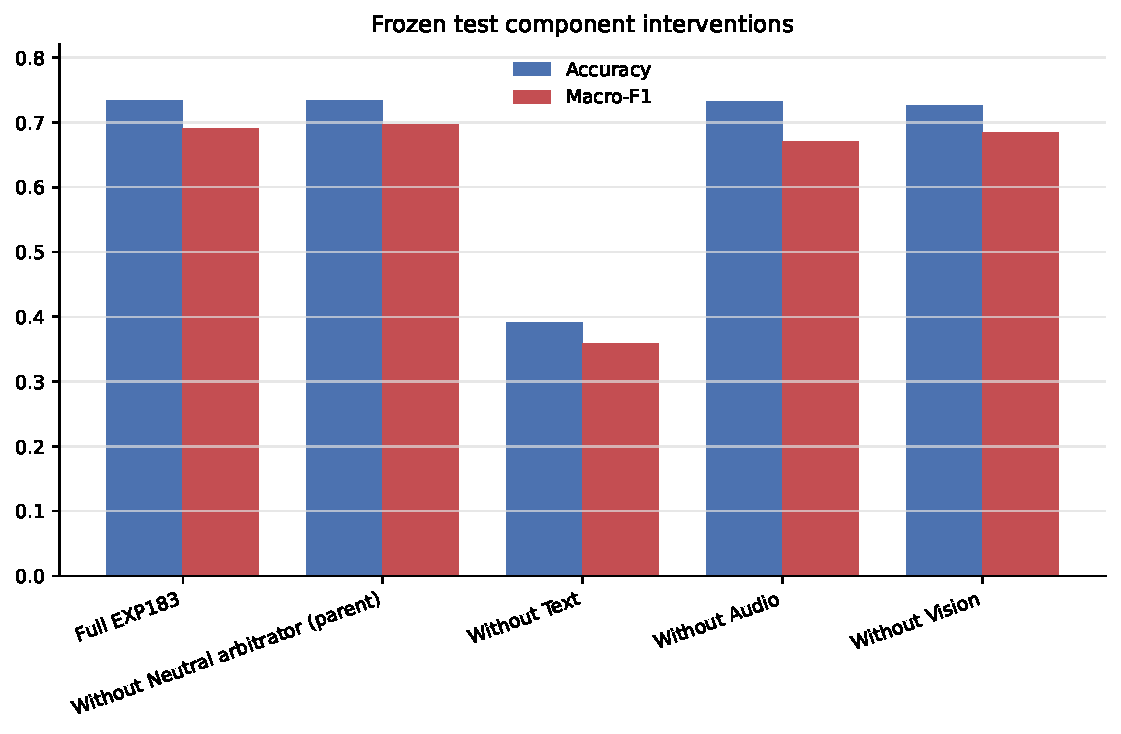
\includegraphics[width=0.49\textwidth]{../figures/fig_q3_ablation.pdf}
  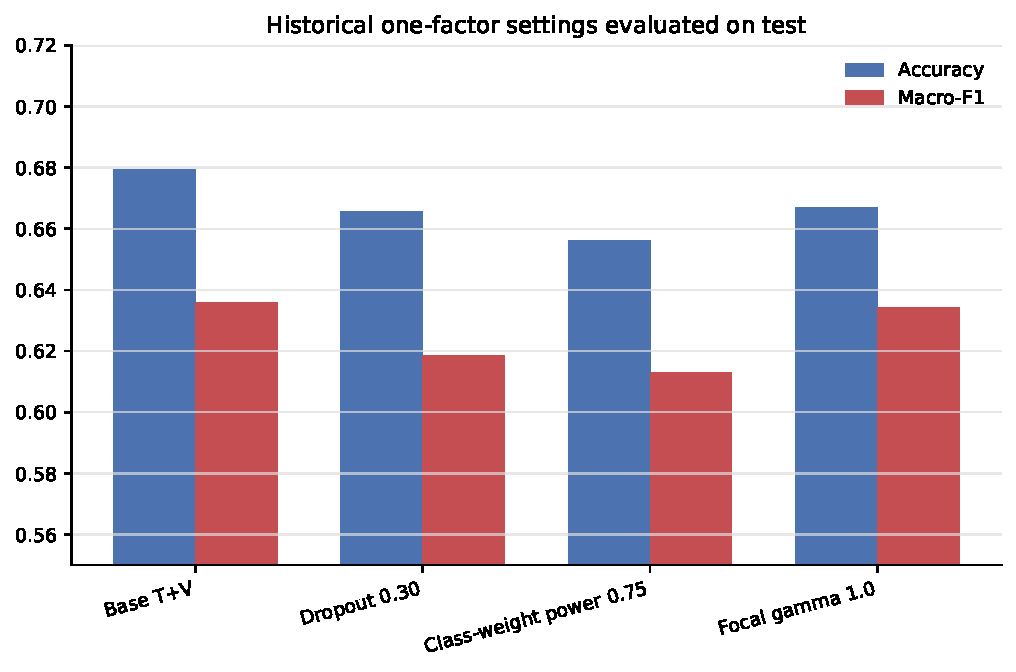
\includegraphics[width=0.49\textwidth]{../figures/fig_q3_sensitivity.pdf}
  \caption{冻结测试集组件干预与历史配置敏感性}
  \label{fig:q3_ablation_sensitivity}
\end{figure}

表~\ref{tab:q3_multitask} 的 EXP003 将回归和 Pearson 权重降低，但分类与回归指标均未形成稳定优势，支持保留均衡联合目标。该对比不是纯 classification-only 实验，因此正文只作“联合损失权重”证据。表~\ref{tab:q3_seed_stability} 的三种子 Focal 实验表现波动，说明单一随机种子的提升不能直接当作稳定结构创新。

\begin{table}[htbp]
\centering
\caption{联合任务损失的真实对比}
\label{tab:q3_multitask}
\small
\resizebox{\textwidth}{!}{%
\begin{tabular}{lrrrr}
\toprule
Loss setting & Acc. & Macro-F1 & MAE & Pearson \\
\midrule
Balanced classification + regression & 0.6657 & 0.6093 & 0.6175 & 0.6988 \\
Classification-focused joint loss & 0.6726 & 0.6135 & 0.6270 & 0.6958 \\
\bottomrule
\end{tabular}%
}
\end{table}

\begin{table}[htbp]
\centering
\caption{随机种子稳定性测试}
\label{tab:q3_seed_stability}
\small
\resizebox{\textwidth}{!}{%
\begin{tabular}{lrrrr}
\toprule
Run & Acc. & Macro-F1 & MAE & Pearson \\
\midrule
exp008\_focal\_gamma1\_seed\_20260924 & 0.6671 & 0.6341 & 0.6123 & 0.7087 \\
exp011\_focal\_gamma1\_seed\_42 & 0.6891 & 0.6597 & 0.5940 & 0.7170 \\
exp012\_focal\_gamma1\_seed\_3407 & 0.6437 & 0.5857 & 0.6407 & 0.6861 \\
\bottomrule
\end{tabular}%
}
\end{table}


\subsection{可解释性生成与可信度检验}

由于最终七成员结构异构，本文采用模型无关但直接作用于最终管线的反事实解释。遮挡模态 \(m\) 后，保留冻结类别 \(\hat c_i\)，计算
\begin{equation}
E_i^m=\frac12|p_{i,\hat c_i}-p_{i,\hat c_i}^{(-m)}|
+\frac12\frac{|\hat y_i-\hat y_i^{(-m)}|}{3},\qquad
\widetilde I_i^m=\frac{E_i^m}{\sum_nE_i^n}.
\label{eq:q3_occlusion_importance}
\end{equation}
主要参考模态定义为 \(m_i^*=\arg\max_m\widetilde I_i^m\)。局部位置使用同样思想：删除模态 \(m\) 的第 \(t\) 个对齐位置，得到
\begin{equation}
e_{i,t}^{m}=\frac12|p_{i,\hat c_i}-p_{i,\hat c_i}^{(-m,t)}|
+\frac12\frac{|\hat y_i-\hat y_i^{(-m,t)}|}{3}.
\label{eq:q3_local_deletion}
\end{equation}

随后按 \(e_{i,t}^m\) 排序，联合删除 top 10\%、20\%、30\% 位置，并与固定随机和 bottom 删除对照。文本位置同时删除比例映射的词片段；音视频位置置零。没有官方时间戳时，位置区间 \([t_1,t_2]\) 按有效长度 \(L_i\) 与视频时长 \(D_i\) 映射为
\begin{equation}
\left[D_i\frac{r(t_1)}{L_i},\;D_i\frac{r(t_2)+1}{L_i}\right],
\label{eq:q3_time_mapping}
\end{equation}
并明确标注为比例近似。视觉关键帧取该近似区间中点，不声称为精确对齐帧。

\subsection{测试集性能评价与错误归因}

表~\ref{tab:q3_main_performance} 给出冻结 test 主结果。EXP183 的 Accuracy 为 0.7331，Macro-F1 为 0.6903，MAE 为 0.5309，Pearson 为 0.7831。相对单一 C$^3$-HAFusion，Accuracy 提升 0.0674，Macro-F1 提升 0.0811，MAE 下降 0.0866。父共识在 test 上事后达到 0.7345/0.6970，但这一信息在 EXP183 冻结后才可见，因此只作为描述性参照，不能用于重新选择正式模型。

\begin{table}[htbp]
\centering
\caption{冻结测试集主模型性能}
\label{tab:q3_main_performance}
\small
\resizebox{\textwidth}{!}{%
\begin{tabular}{lrrrrrrrr}
\toprule
Model & Acc. & Macro-F1 & Weighted-F1 & Bal. Acc. & MAE & RMSE & Bias & Pearson \\
\midrule
Single C3-HAFusion & 0.6657 & 0.6093 & 0.6598 & 0.6092 & 0.6175 & 0.8356 & 0.0570 & 0.6988 \\
EXP169 parent consensus & 0.7345 & 0.6970 & 0.7309 & 0.6958 & 0.5309 & 0.7198 & 0.0073 & 0.7831 \\
EXP183 frozen deployment & 0.7331 & 0.6903 & 0.7273 & 0.6890 & 0.5309 & 0.7198 & 0.0073 & 0.7831 \\
\bottomrule
\end{tabular}%
}
\end{table}

\begin{table}[htbp]
\centering
\caption{冻结测试集分类别性能}
\label{tab:q3_per_class}
\small
\resizebox{\textwidth}{!}{%
\begin{tabular}{lrrrr}
\toprule
Class & Precision & Recall & F1 & Support \\
\midrule
Negative & 0.7534 & 0.7971 & 0.7746 & 207 \\
Neutral & 0.5504 & 0.4494 & 0.4948 & 158 \\
Positive & 0.7836 & 0.8204 & 0.8016 & 362 \\
\bottomrule
\end{tabular}%
}
\end{table}


测试混淆矩阵见图~\ref{fig:q3_confusion}。Negative 和 Positive F1 分别为 0.7746 与 0.8016，而 Neutral F1 为 0.4948；Neutral 仅正确识别 71/158，其中 59 个被判为 Positive。全部 727 个样本中，145 个错误属于 Neutral 边界，49 个属于正负极性反转。后者的平均绝对回归误差为 1.3158，是最严重的联合错误。

\begin{figure}[htbp]
  \centering
  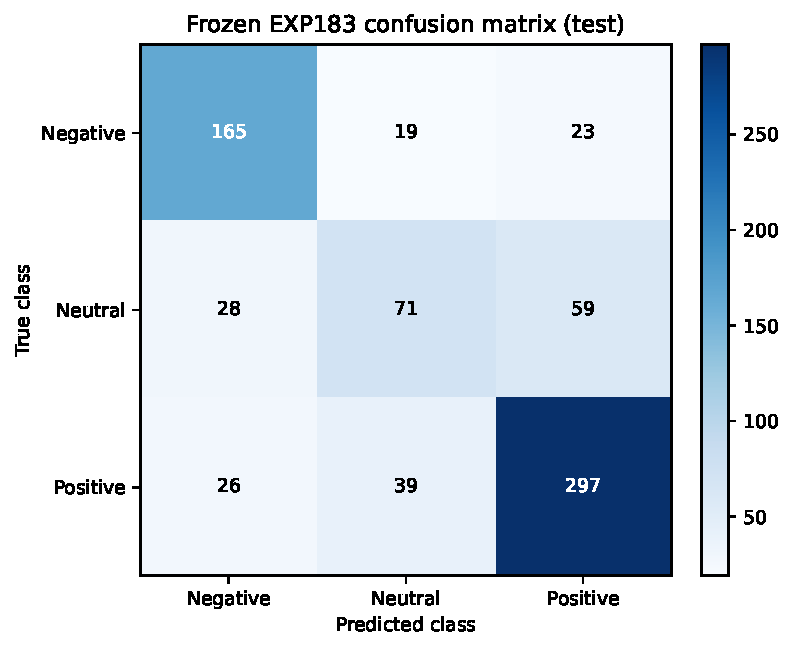
\includegraphics[width=0.68\textwidth]{../figures/fig_q3_confusion_matrix.pdf}
  \caption{冻结 EXP183 在测试集上的混淆矩阵}
  \label{fig:q3_confusion}
\end{figure}

\begin{figure}[htbp]
  \centering
  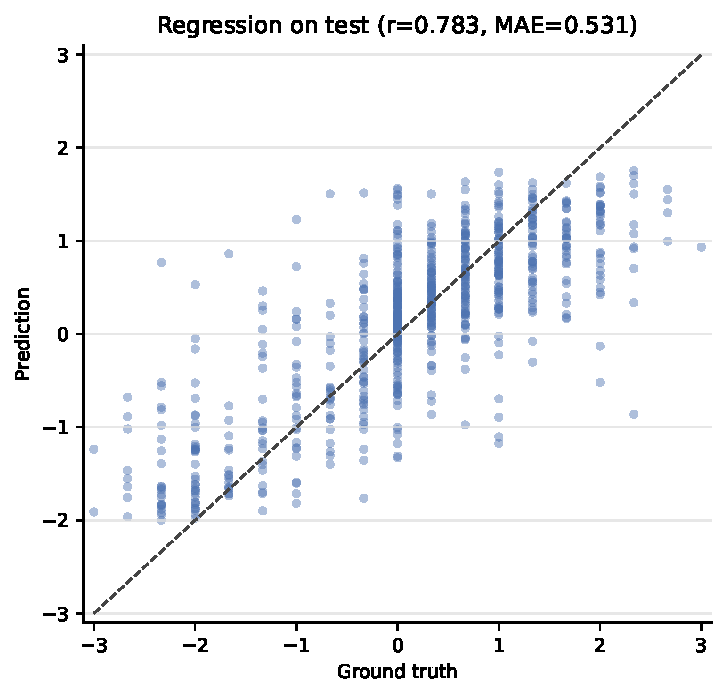
\includegraphics[width=0.49\textwidth]{../figures/fig_q3_regression_scatter.pdf}
  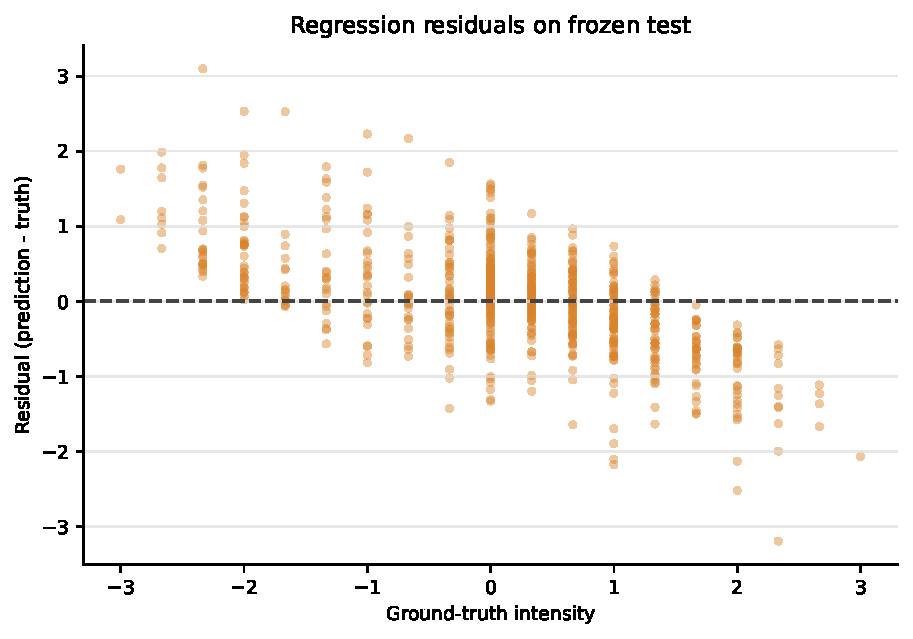
\includegraphics[width=0.49\textwidth]{../figures/fig_q3_residual.pdf}
  \caption{冻结测试集连续强度预测与残差}
  \label{fig:q3_regression}
\end{figure}

用 validation 独立选择 \(\varepsilon=0.149\) 将回归值映射到三类后，test 分类--回归一致率为 0.8762，回归符号单独分类的 test Accuracy 为 0.7345。该指标仅用于诊断，不改变正式分类输出。

\subsection{模态作用差异、消融与解释结果}

\begin{table}[htbp]
\centering
\caption{单模态与模态组合的测试集结果}
\label{tab:q3_modality_combinations}
\small
\resizebox{\textwidth}{!}{%
\begin{tabular}{lrrrr}
\toprule
Modalities & Acc. & Macro-F1 & MAE & Pearson \\
\midrule
T+A+V & 0.6602 & 0.6136 & 0.6109 & 0.7043 \\
T & 0.6671 & 0.6271 & 0.6240 & 0.6975 \\
A & 0.4553 & 0.3722 & 0.8782 & 0.1885 \\
V & 0.4360 & 0.3943 & 0.8694 & 0.2326 \\
T+A & 0.6685 & 0.6245 & 0.6153 & 0.6988 \\
T+V & 0.6657 & 0.6241 & 0.6168 & 0.7020 \\
A+V & 0.4525 & 0.4113 & 0.8518 & 0.2770 \\
\bottomrule
\end{tabular}%
}
\end{table}

\begin{table}[htbp]
\centering
\caption{冻结测试集模态遮挡结果}
\label{tab:q3_occlusion}
\small
\resizebox{\textwidth}{!}{%
\begin{tabular}{lrrrrr}
\toprule
Condition & Acc. & Macro-F1 & MAE & Pearson & Flip rate \\
\midrule
full & 0.7331 & 0.6903 & 0.5309 & 0.7831 & 0.0000 \\
without\_text & 0.3906 & 0.3594 & 0.8689 & 0.2394 & 0.5433 \\
without\_audio & 0.7318 & 0.6710 & 0.5350 & 0.7841 & 0.0825 \\
without\_vision & 0.7263 & 0.6843 & 0.5339 & 0.7783 & 0.0757 \\
\bottomrule
\end{tabular}%
}
\end{table}


在同一冻结 HAFusion 中，文本单模态的 test Accuracy/Macro-F1 为 0.6671/0.6271，明显强于 Audio 的 0.4553/0.3722 和 Vision 的 0.4360/0.3943。对最终 EXP183 做全体 test 遮挡后，移除文本使指标降至 0.3906/0.3594；移除语音为 0.7318/0.6710；移除视觉为 0.7263/0.6843。这说明文本提供主要判别证据，音视频承担边界修正和可信度补充。

全局平均作用程度为 Text 0.7398、Audio 0.1362、Vision 0.1240；主要参考模态分别占 84.18\%、8.94\% 和 6.88\%。Neutral 样本的平均作用程度为 0.6025/0.2344/0.1631，语音和视觉占比高于强极性样本，说明弱情感边界更依赖非文本补充。

\begin{figure}[htbp]
  \centering
  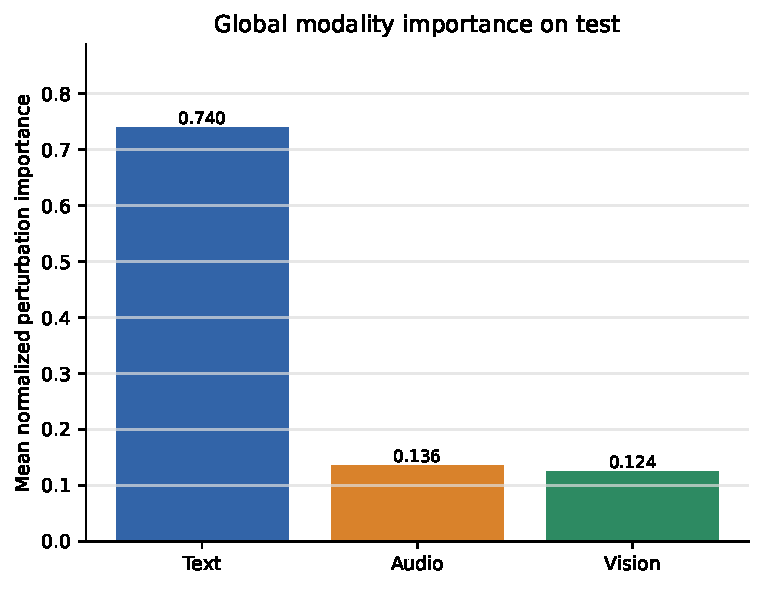
\includegraphics[width=0.49\textwidth]{../figures/fig_q3_modality_global.pdf}
  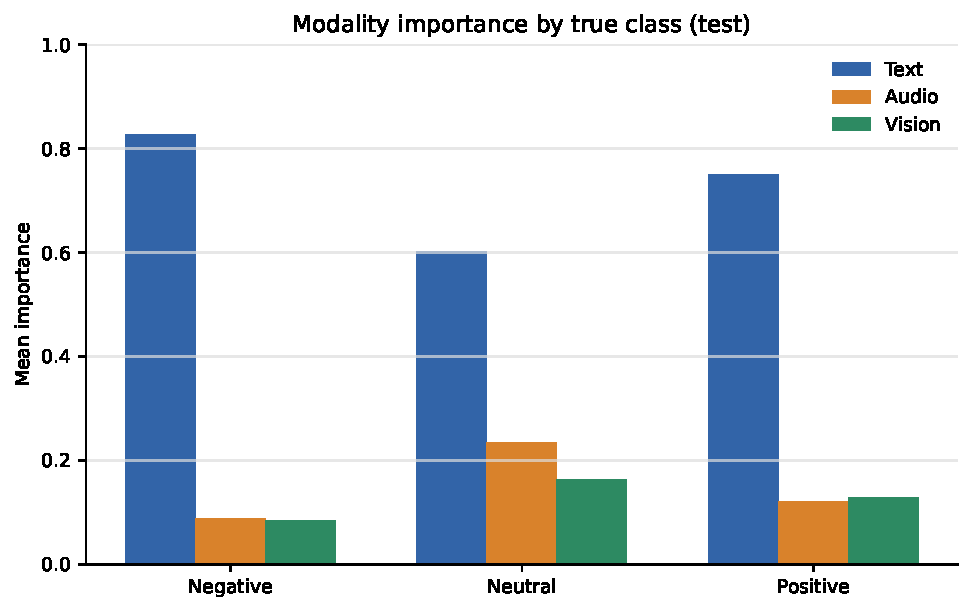
\includegraphics[width=0.49\textwidth]{../figures/fig_q3_modality_class.pdf}
  \caption{冻结测试集的整体与分类别模态作用程度}
  \label{fig:q3_modality_importance}
\end{figure}

\begin{figure}[htbp]
  \centering
  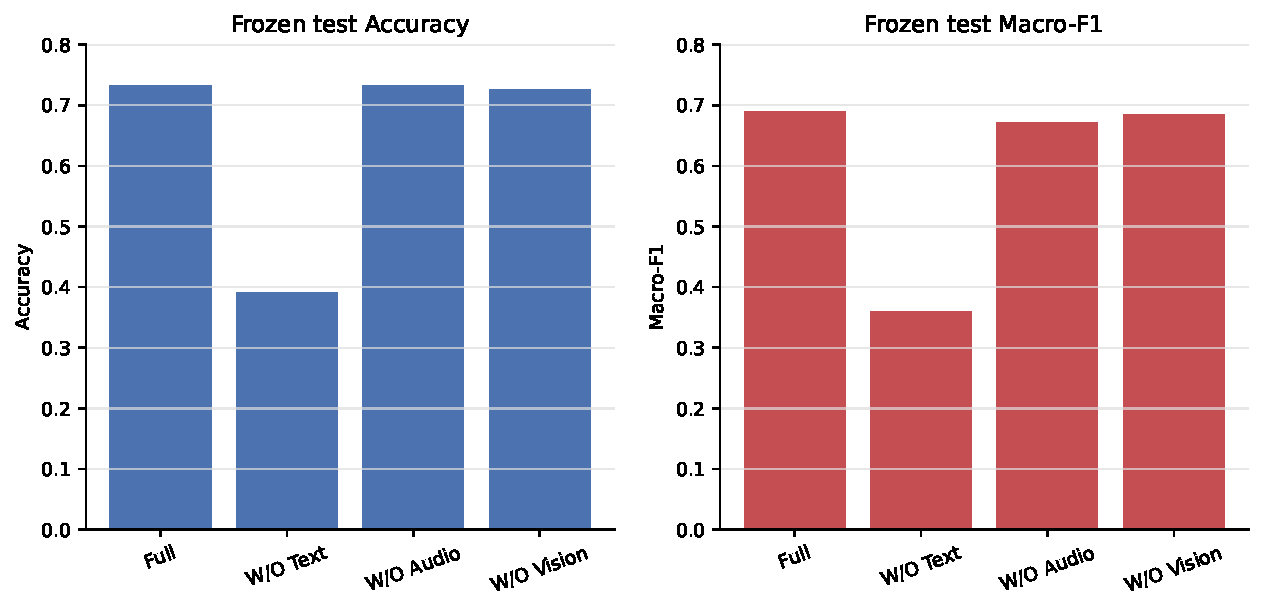
\includegraphics[width=0.64\textwidth]{../figures/fig_q3_occlusion.pdf}
  \caption{冻结测试集最终部署的模态遮挡实验}
  \label{fig:q3_occlusion}
\end{figure}

对六个按真实类别和预测对错分层选择的测试案例，top 局部证据删除引起的冻结类别置信度变化整体高于随机和 bottom 删除。该实验用于说明案例解释的忠实性，不把六个案例外推成全体 test 统计。

\begin{table}[htbp]
\centering
\caption{选定测试案例的局部证据删除结果}
\label{tab:q3_evidence_deletion}
\small
\resizebox{\textwidth}{!}{%
\begin{tabular}{lrrrr}
\toprule
Modality & Ratio & Strategy & Confidence drop & Flip rate \\
\midrule
audio & 0.1000 & bottom & 0.0101 & 0.1667 \\
audio & 0.1000 & random & -0.0021 & 0.0000 \\
audio & 0.1000 & top & -0.0012 & 0.0000 \\
audio & 0.2000 & bottom & 0.0231 & 0.1667 \\
audio & 0.2000 & random & 0.0000 & 0.0000 \\
audio & 0.2000 & top & 0.0102 & 0.1667 \\
audio & 0.3000 & bottom & 0.0253 & 0.1667 \\
audio & 0.3000 & random & 0.0256 & 0.1667 \\
audio & 0.3000 & top & 0.0160 & 0.1667 \\
text & 0.1000 & bottom & -0.0052 & 0.0000 \\
text & 0.1000 & random & 0.1331 & 0.1667 \\
text & 0.1000 & top & 0.1918 & 0.3333 \\
text & 0.2000 & bottom & -0.0153 & 0.0000 \\
text & 0.2000 & random & 0.1189 & 0.1667 \\
text & 0.2000 & top & 0.2059 & 0.3333 \\
text & 0.3000 & bottom & -0.0230 & 0.0000 \\
text & 0.3000 & random & 0.1235 & 0.3333 \\
text & 0.3000 & top & 0.2420 & 0.3333 \\
vision & 0.1000 & bottom & -0.0134 & 0.0000 \\
vision & 0.1000 & random & -0.0126 & 0.0000 \\
vision & 0.1000 & top & -0.0010 & 0.0000 \\
vision & 0.2000 & bottom & 0.0106 & 0.1667 \\
vision & 0.2000 & random & -0.0028 & 0.1667 \\
vision & 0.2000 & top & -0.0039 & 0.0000 \\
vision & 0.3000 & bottom & 0.0108 & 0.1667 \\
vision & 0.3000 & random & -0.0043 & 0.1667 \\
vision & 0.3000 & top & -0.0041 & 0.0000 \\
\bottomrule
\end{tabular}%
}
\end{table}


\begin{figure}[htbp]
  \centering
  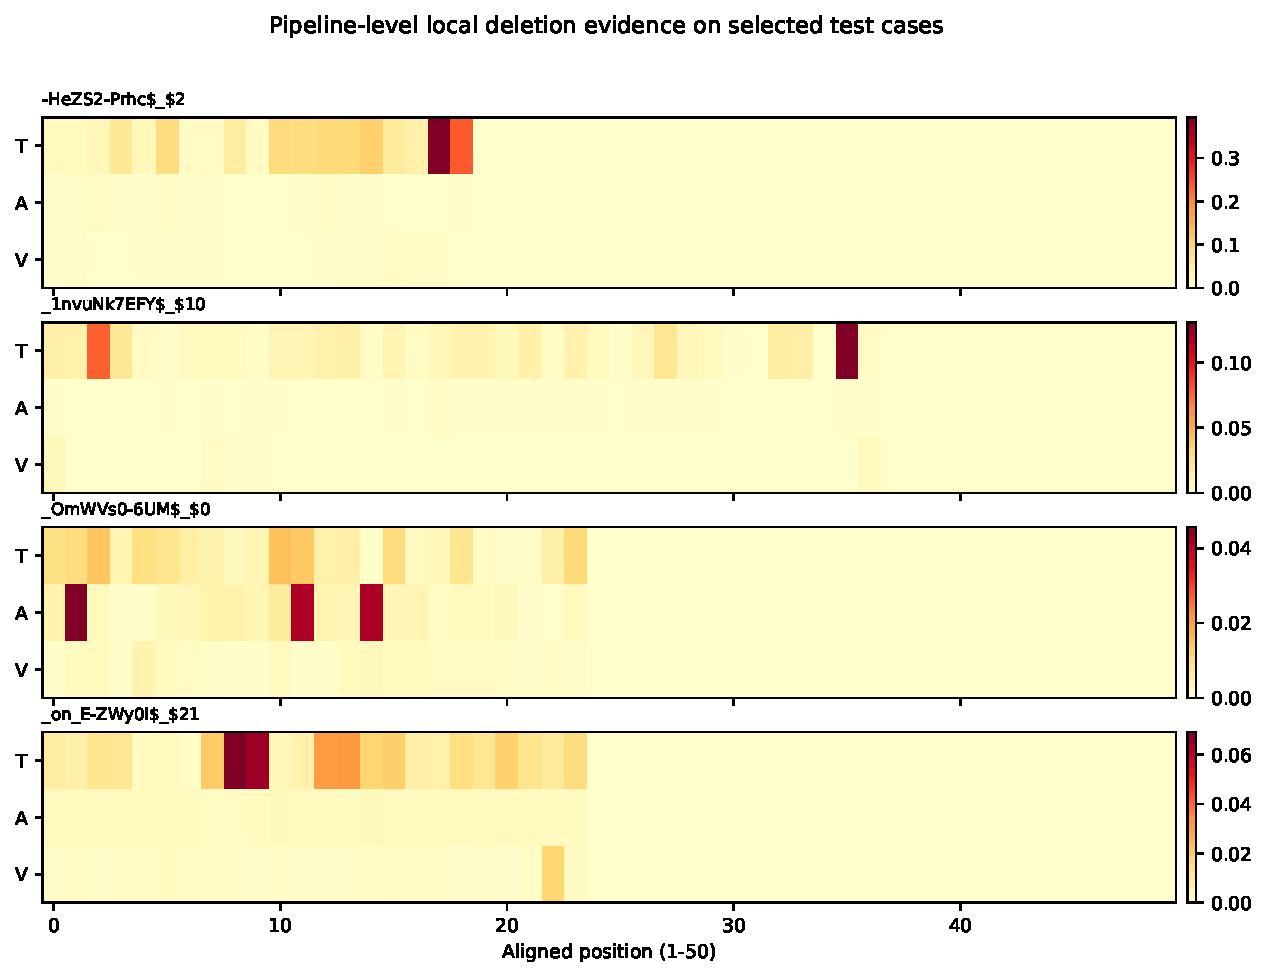
\includegraphics[width=0.49\textwidth]{../figures/fig_q3_evidence_heatmap.pdf}
  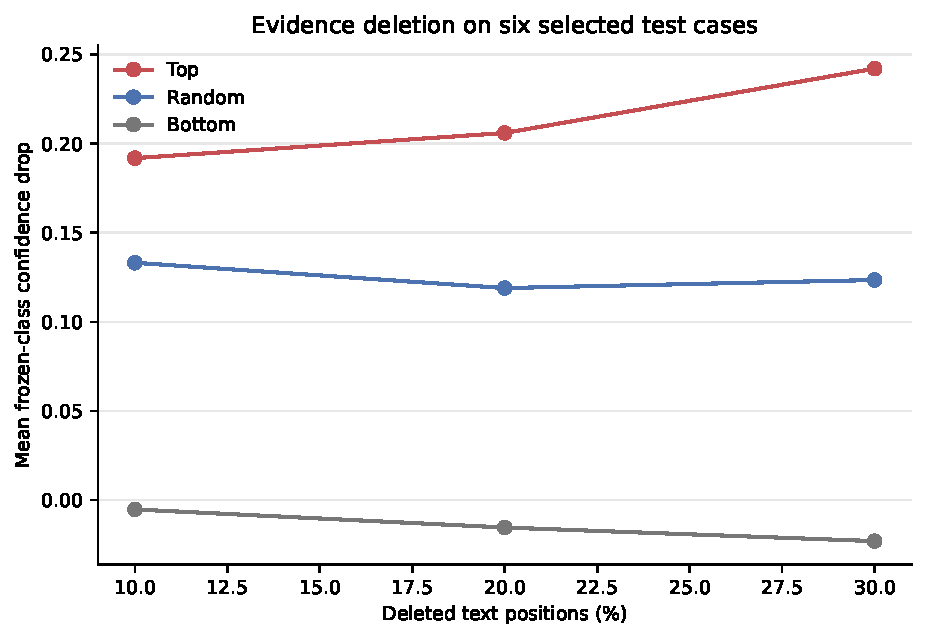
\includegraphics[width=0.49\textwidth]{../figures/fig_q3_evidence_deletion.pdf}
  \caption{典型测试案例的局部删除证据与忠实性对照}
  \label{fig:q3_local_evidence}
\end{figure}

\subsection{典型样本解释卡分析}

\begin{table}[htbp]
\centering
\caption{典型测试样本解释结果}
\label{tab:q3_cases}
\small
\resizebox{\textwidth}{!}{%
\begin{tabular}{lrrrrr}
\toprule
ID & Truth & Prediction & Intensity & Dominant & Key text \\
\midrule
-HeZS2-Prhc\$\_\$2 & Positive & Negative & -0.2531 & vision & not great. | overall as solid \\
\_1nvuNk7EFY\$\_\$10 & Negative & Negative & -0.9724 & text & overfishing level. | alarming report found | five times the \\
\_OmWVs0-6UM\$\_\$0 & Neutral & Neutral & 0.2914 & audio & As part of | the year | France. \\
\_on\_E-ZWy0I\$\_\$21 & Positive & Positive & 1.1998 & text & debt, kick some | butt and get | motivated \\
\_on\_E-ZWy0I\$\_\$3 & Neutral & Negative & -1.0801 & text & huge problem that | on hundreds, | thousands of \\
\_on\_E-ZWy0I\$\_\$12 & Negative & Neutral & 0.1607 & text & reach out to us and | you a free credit | paid all of \\
\bottomrule
\end{tabular}%
}
\end{table}


正确极性样本通常具有集中且方向明确的文本证据；例如 Negative 正确样本的文本作用程度达到约 0.93。Neutral 正确样本中，Audio 成为主要模态，说明非文本信息可在缺少强极性词时提供补充。错误样本 \texttt{-HeZS2-Prhc\$\_\$2} 的真实类别为 Positive，而模型预测 Negative；其 T/A/V 作用程度约为 0.229/0.335/0.436，视觉成为主要模态，关键文本同时出现 ``not great'' 与 ``overall as solid''，体现了跨模态及文本内部冲突。该案例说明高解释性不能保证预测必然正确，但能暴露错误由何种证据驱动。

\begin{figure}[htbp]
  \centering
  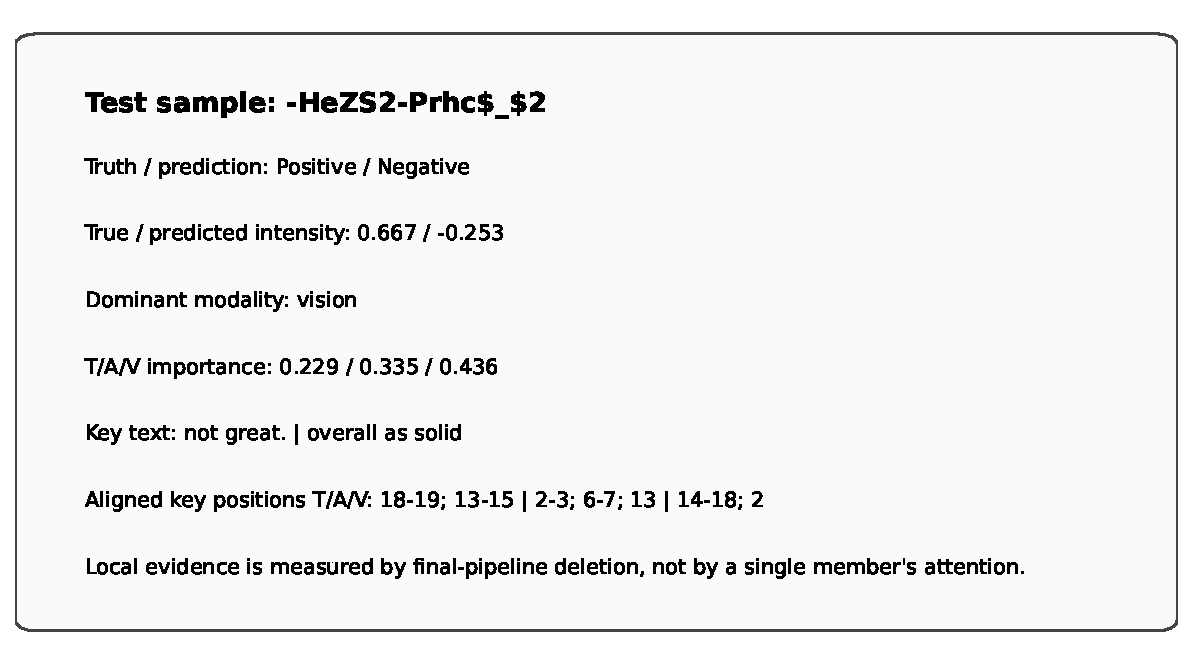
\includegraphics[width=0.9\textwidth]{../figures/fig_q3_explanation_card.pdf}
  \caption{典型测试错误样本的解释卡}
  \label{fig:q3_case_card}
\end{figure}

\subsection{附件4全量预测与解释结果}

冻结 EXP183 对附件4的 20 个无标签样本执行一次性推理，没有利用附件4调整任何模型项。预测类别为 Negative 6、Neutral 3、Positive 11；20/20 样本找到原视频。主要参考模态为 Text 18、Vision 2、Audio 0，平均作用程度为 0.7735/0.0767/0.1497。

附件结果表包含样本编号、三类概率、预测强度、三模态作用程度、主要模态、文本/语音/视觉关键位置、关键文本、音频/视觉比例时间区间和关键帧路径。每个样本还完成单位置删除和 top/random/bottom 联合删除。附件4没有真实标签，因此不报告 Accuracy、F1、MAE 或 Pearson。

\begin{table}[htbp]
\centering
\caption{附件4预测结果示例}
\label{tab:q3_attachment4}
\small
\resizebox{\textwidth}{!}{%
\begin{tabular}{lrrrr}
\toprule
ID & Class & Intensity & Dominant & Key text \\
\midrule
01 & Positive & 0.3716 & text & is essential to | ensuring the | replacing the \\
02 & Positive & 0.5751 & text & not | other’s happiness | each \\
03 & Negative & -0.5365 & text & don't take | into account, | think is \\
04 & Positive & -0.0681 & text & goodbye?] Absolutely not. | should I | cheering \\
05 & Positive & 0.8584 & text & Marketing. | Hi, my | Chloe, video \\
06 & Positive & 0.7609 & text & check out this movie | If you're a | might want \\
07 & Positive & 0.9243 & text & attendees “enthusiastically discussed the | make it succeed and | Baadke reports in \\
08 & Neutral & 0.2657 & vision & brings us to | Design Grand Challenge | tonight, the \\
09 & Negative & -1.9893 & text & not recommend | not like \\
10 & Negative & -1.5473 & text & terrible | (umm) \\
\bottomrule
\end{tabular}%
}
\end{table}


\subsection{问题三小结}

本文建立了两层可解释多模态情感预测方案：基础 C$^3$-HAFusion 在对齐位置、模态对冲突和动态贡献三个层次形成可加证据；最终 EXP183 通过七成员固定共识与 Neutral 真实性仲裁提升泛化性能。冻结测试集结果为 Accuracy 0.7331、Macro-F1 0.6903、MAE 0.5309、Pearson 0.7831。全体 test 模态遮挡证实文本总体主导，Neutral 边界更依赖音视频补充；局部删除进一步验证典型案例的关键位置确实影响最终输出。最后，附件4 20 个样本均已输出极性、强度、全局作用程度、局部证据和视频关键帧，从而形成从预测到解释再到复核的完整闭环。
